\section{Learning the kernel: the Laplace chain}
\label{sec:laplace}

\note{The largest section (33:47): ``the heart of the proposal is EM on Markov chains'' (29:29). The whole
comparison with a network that has locality (CNN) and one that has none (MLP), then breaking Markovianity, in the main
text.}

\subsection{Expectation--maximisation through BP}
\label{sec:em}

\begin{figure}[t]
  \centering
  \begin{tikzpicture}[
    box/.style={draw,thick,align=center,font=\small,minimum height=9mm,inner sep=3pt,text width=1.6cm},
    data/.style={box,fill=black!8},
    arr/.style={-{Stealth[length=2mm]},thick},
    lab/.style={font=\small,align=center}]
  \node[font=\small\bfseries,anchor=west] at (-1.1,1.0) {learn};
  \node[data] (d) at (0,0) {noisy\\ sequences};
  \node[box] (p) at (3.1,0) {pair\\ posteriors};
  \node[box] (k) at (6.2,0) {kernel $K_\theta$};
  \draw[arr] (d) -- node[above,lab]{BP} node[below,lab]{E-step} (p);
  \draw[arr] (p) -- node[above,lab]{refit} node[below,lab]{M-step} (k);
  \draw[arr] (k.north) to[out=160,in=20] node[above,lab]{repeat} (d.north);
  \node[font=\small\bfseries,anchor=west] at (-1.1,-1.55) {use};
  \node[data] (x) at (0,-2.5) {noisy\\ sequence $x$};
  \node[box] (m) at (3.1,-2.5) {$\mathbb{E}[a\mid x]$};
  \node[box] (s) at (6.2,-2.5) {score $S_t(x)$};
  \draw[arr] (x) -- node[below,lab]{BP} (m);
  \draw[arr] (m) -- (s);
  \draw[thick,dashed,-{Stealth[length=2mm]}] (k.south) -- (6.2,-1.25) -| (1.55,-2.47);
\end{tikzpicture}

  \caption{\note{Learn: BP (E-step) gives pair posteriors, the refit (M-step) gives $K_\theta$, repeat. Use: BP with
  $K_\theta$ gives $\E[a\mid x]$, hence the score. Slide 11.}}
  \label{fig:em-loop}
\end{figure}

\note{J\'er\^ome (50:20): explain EM more, in the logic of the gradient of an expectation: BP gives the expectation;
the kernel is a controlled function of $\theta$; take the gradient of the expectation over $\theta$ and follow it, on a
given set of examples. E-step: pair posteriors $\xi_k(a,a')$, summed into expected counts $\Xi$. M-step: raise
$Q(\theta)=\iint\Xi\log K_\theta$. Fisher's identity: $\nabla Q=\nabla\log p_\theta(x)$ at $\theta_{\rm old}$, so the
likelihood never decreases (23:38).}

\note{Say explicitly (his worry at 39:37--41:27): there is NO backpropagation through BP. BP enters only through
$\Xi$, constant during the M-step; autograd only goes through $K_\theta$ and its grid normaliser
(\texttt{energy\_kernel.py}, E55). Also: the noise level is only in the E-step, so no noise schedule is needed to
learn the kernel.}

\subsection{Kernel families}
\label{sec:families}

\begin{figure*}[t]
  \centering
  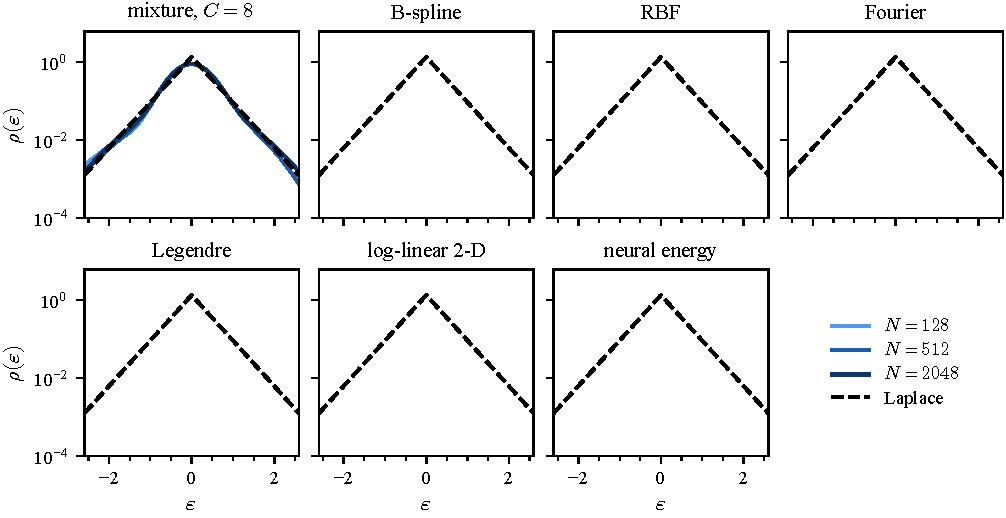
\includegraphics{fig_families}
  \caption{\note{Thesis Fig.~6.3 for every family (37:41): learned innovation law at $N=128$, $512$, $2048$ against
  the Laplace truth (dashed). Mixture from exp\_18; the other six from E56 (pending).}}
  \label{fig:families}
\end{figure*}

\note{J\'er\^ome (22:15, 26:41): why would the kernel be a mixture of $C$ Gaussians? Families he named: truncated
Fourier series (28:18), polynomials, Gaussian RBF, Mat\'ern (29:29). Put the series on $\log K$, not on $K$: positive
kernel, concave M-step. Local bases (spline, RBF) can make the kink; global (Fourier, Legendre) only by oscillating.
Shift families vs agnostic ones (log-linear 2-D, neural energy kernel: 2-layer MLP, 13:45, 39:37).}

\note{Mixture numbers (fig\_em\_innovation, App.~B): $\alpha$ within $0.1\%$ from $N=512$ ($2.4\%$ at $128$);
excess kurtosis only within $6$--$25\%$.}

\subsection{Against neural denoisers}
\label{sec:networks}

\begin{figure}[t]
  \centering
  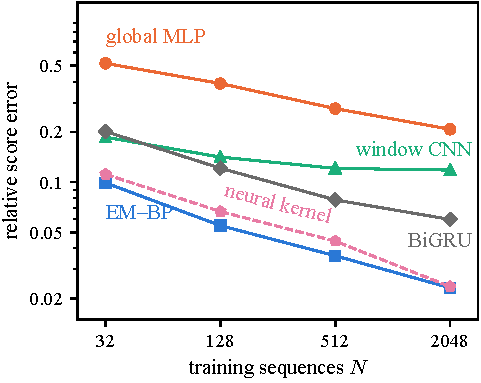
\includegraphics{fig_value_of_structure}
  \caption{\note{Slide 14 as one plot (21:25): EM--BP, global MLP, window CNN, and BiGRU (the best of six from
  $N=128$). Same test sequences, 16 seeds.}}
  \label{fig:value-of-structure}
\end{figure}

\begin{figure}[t]
  \centering
  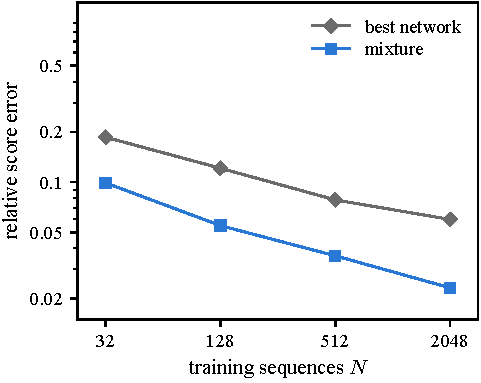
\includegraphics{fig_families_error}
  \caption{\note{Every kernel family against $N$, best network for reference. E56 (pending).}}
  \label{fig:families-error}
\end{figure}

\note{J\'er\^ome (21:25): this is where ML people will complain, so be careful. Networks: DSM on CLEAN sequences
(an advantage), screened on dev seeds, validation checkpoint; EM sees one noisy copy of each sequence.}

\note{Numbers (paired E02a/E03, mean per-seed ratio network/EM--BP, $N=32,128,512,2048$): MLP $5.79, 7.95, 7.88,
9.85$; window CNN $2.07, 2.87, 3.45, 5.58$; BiGRU $2.22, 2.45, 2.24, 2.83$. Honest headline: best network at each $N$,
$2.1$--$2.8\times$. EM--BP error $0.099\to0.023$; CNN $0.19\to0.12$ (flat: the window floor of Sec.~3). These replace
the thesis's $6.6$--$10.9\times$ and $2.3$--$6.1\times$.}

\subsection{Step efficiency}
\label{sec:steps}

\begin{figure*}[t]
  \centering
  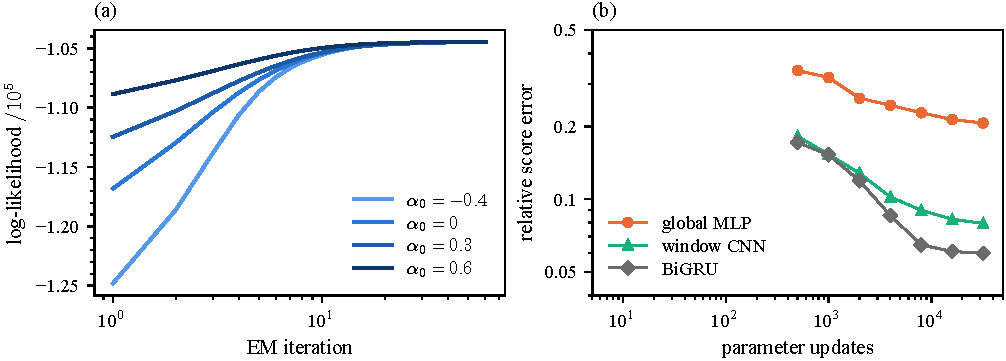
\includegraphics{fig_em_dynamics}
  \caption{\note{(a) EM log-likelihood against iteration, four starts. (b) Validation score error against parameter
  updates: EM iterations (E56, pending) and SGD steps (E03), $N=2048$.}}
  \label{fig:em-dynamics}
\end{figure*}

\note{J\'er\^ome (22:15, 23:50): dynamics curves; the claim is ``not only sample efficient, also step efficient''.
Wall-clock is less important (23:50). Careful: he expects $\sim10$ steps (25:16); measured: likelihood plateau in
$\sim20$ iterations, $\alpha$ settles in a median of 80 updates, the shape in 229 (tail 638) (thesis exp\_27). Still
2--3 orders fewer than the networks' $10^3$--$3\times10^4$ SGD steps. Per EM iteration: 3--6.6\,s at $N=2048$, one
CPU thread (E56 timing).}

\subsection{When the data are not Markov}
\label{sec:nonmarkov}

\begin{figure}[t]
  \centering
  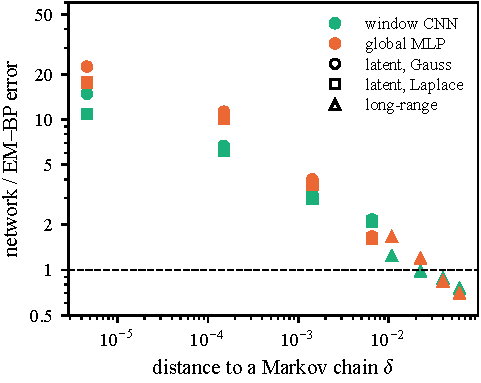
\includegraphics{fig_nonmarkov}
  \caption{\note{Network / EM--BP error against $\delta$, the distance per site to the closest first-order chain.
  Global latent (Gaussian and Laplace) and long-range couplings. Below 1 the network wins.}}
  \label{fig:nonmarkov}
\end{figure}

\note{J\'er\^ome (32:51--33:47): break the Markovianity and see how long it stays good, in the main text. Global latent
$a=(y+\beta g)/\sqrt{1+\beta^2}$; long-range $Q_{\rm AR}+\gamma Q_{\rm long}$. Numbers: at $\delta\approx5\times10^{-6}$
CNN $11$--$15\times$ worse, MLP $18$--$22\times$; break-even $\delta^\star\approx1$--$2\times10^{-2}$ (CNN),
$2$--$4\times10^{-2}$ (MLP); $\hat\alpha$ $0.848\to0.939$ at $\beta=1$. Second-order chain: not run yet.}
